
Ensembler is implemented in Python3\cite{VanRossum2009} and available on GitHub\cite{Github2020}  (\textit{\hyperlink{https://github.com/rinikerlab/Ensembler}{rinikerlab/Ensembler}}). 
The repository is based on the template of the MolSSI cookie-cutter\cite{Naden2018} and comprises a code folder, an example folder for tutorials, example models contained in the provided Jupyter notebooks,\cite{Kluyver2016} an automatic pytest suite,\cite{Krekel2004} and the automatically generated sphinx \cite{Brandl2008} documentation. 
The code is continuously integrated via GitHub Actions,\cite{githhubAction20} providing information about code quality, test correctness, test coverage, and generation of an up-to-date documentation. 
Ensembler uses only open-source packages like the SciPy library\cite{Virtanen2020, VanDerWalt2011, Meurer2017, Mckinney2010, Hunter2007} and Jupyter notebooks.\cite{Kluyver2016} 
In the following, a user and a developer perspective are provided for the code structure. 


\begin{figure}[ht]
	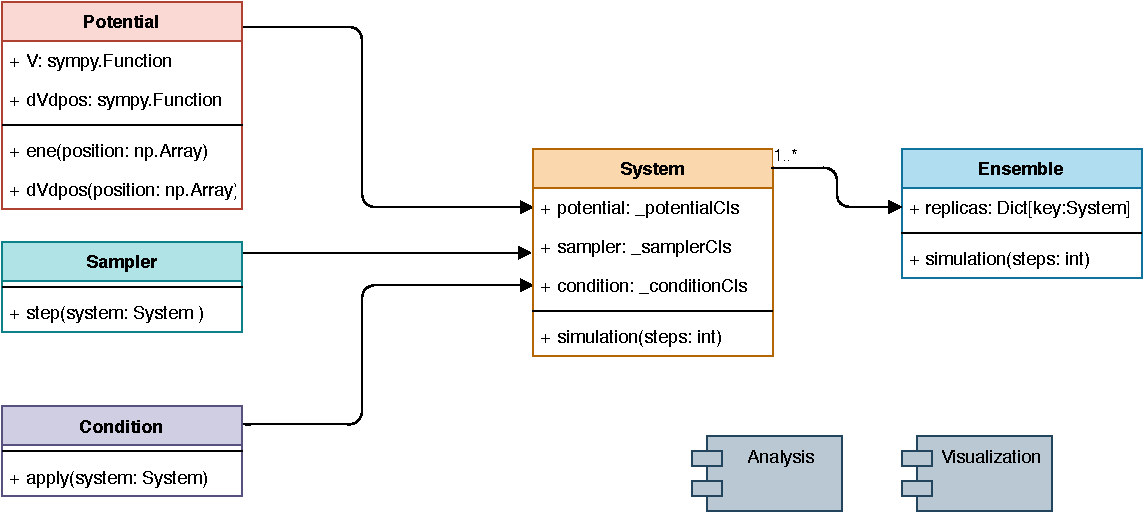
\includegraphics[width=\textwidth]{fig/implementation/export.pdf}
	\caption{Unified modeling language (UML) class diagram of the five Ensembler base classes. The \textit{potential class} defines the potential-energy functions to be explored and generates the required derivatives automatically (Figure \ref{fig:code_example_potential}). The implementation of a \textit{potential class} (red) is based on the symbolic mathematical language of SymPy.\cite{Meurer2017} The \textit{sampler classes} (cyan) are used for the sampling of potential-energy functions. \textit{Condition classes} (purple) can have different functions, e.g. application of periodic boundary conditions,\cite{Cheatham1995, Leach2001} thermostats, or restraints. The \textit{system classes} (orange) serve as the scaffold for the potential, sampler, and condition classes. In this structure, all components, parameters, and the results of a simulation are stored. The \textit{Ensemble class} (blue) can be used to perform advanced simulation techniques, e.g. using multiple walkers that explore the energy landscapes of the same or different systems as in replica-exchange approaches.\cite{Sugita1999, Sugita2000, Yamauchi2017} The \textit{analysis package} includes free-energy methods such as the Zwanzig equation\cite{Zwanzig1954} or BAR\cite{Bennett1976}. A set of visualization functions is provided in the \textit{visualization package} to enable an intuitive way of inspecting simulations or exploring potentials-energy functions. This includes plots, animations, and interactive widgets.}
	\label{fig:UML-Diagramm}
\end{figure}


%-------------------------------------------------------
\subsection{User level}
%-------------------------------------------------------
 A simulation model in Ensembler consists of a potential class, a sampler class, and a system class wrapping the potential and the sampler (Figure~\ref{fig:UML-Diagramm}), and provides control over the simulation approach. 
Additionally, multiple condition classes can be added that directly influence the simulation (e.g. periodic boundary condition\cite{Cheatham1995, Leach2001} or  thermostatting\cite{Andersen1980}). 
After the construction of the system, the simulation can be started directly with the \textit{simulate} function. 
The resulting trajectory is in the form of a Pandas data frame.\cite{Mckinney2010} The trajectory is thus easily compatible with other packages like NumPy\cite{VanDerWalt2011} or scikit-learn\cite{scikit-learn} and can be stored in different formats, e.g. as .csv or .hf5 file. The system itself can be stored directly via the save function using serialization of the object with the Python package pickle.
In most cases, only a few additional lines are needed to go from simple simulation technique to more advanced one, as shown below. 

%-------------------------------------------------------
\subsection{Developer level}
%-------------------------------------------------------
The code of Ensembler is built on five interface-like base classes that allow extensive use of the inheritance concept and polymorphism \cite{Stroustrup1995} throughout the package.
These fundamental classes are \textit{potential}, \textit{sampler}, \textit{condition}, \textit{system}, and \textit{ensemble} (Figure \ref{fig:UML-Diagramm}), which can be grouped into three layers.
\textit{Potential}, \textit{sampler}, and \textit{condition classes} form the primary layer, providing different techniques to be used as components in a simulation. 
\textit{Potential classes} provide the potential-energy functions in a symbolic form using SymPy,\cite{Meurer2017} enabling automatic on-the-fly derivation and simplification of the potential-energy function. 
\textit{Sampler classes} are used to explore the potential-energy function (e.g. conjugate gradient,\cite{Hestenes1952} Metropolis MC,\cite{Hastings1970} or leap-frog\cite{VanGunsteren1988} integration). A new method can easily be implemented by inheriting from the \textit{sampler class} and overwriting a single function called \textit{step}. 
Finally, \textit{condition classes} provide additional functionalities such as thermostatting\cite{Andersen1980} and periodic boundary conditions\cite{Cheatham1995, Leach2001}). New techniques can be implemented by inheriting the base \textit{condition class} and overwriting the function \textit{apply}.
In the second layer, the first-layer components are wrapped into one \textit{system class} that executes the simulation(s) and manages the input and output. 
An optional higher-order layer is available in form of the \textit{ensemble class}, which allows the user to perform simulations with replica exchange.\cite{Sugita1999, Sugita2000, Yamauchi2017, Sidler2016}
If additional parameters are needed in a newly designed class, the constructor of the new child class can be adapted but must call the parent constructor.
